\begin{figure}[ht]
\centering
\subfigure[Moduł sprężystości objętościowej]{%
    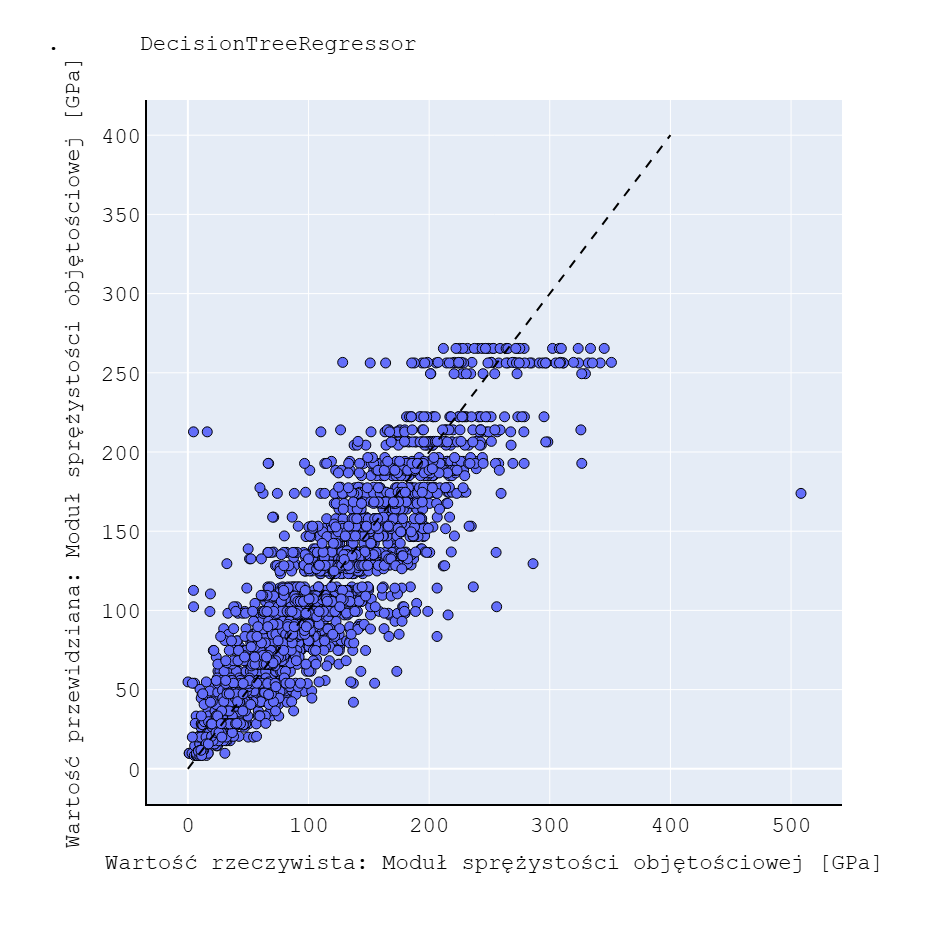
\includegraphics[width=0.48\textwidth]{images/figures/newplot (7).png}
}
\subfigure[Moduł sprężystości poprzecznej]{%
    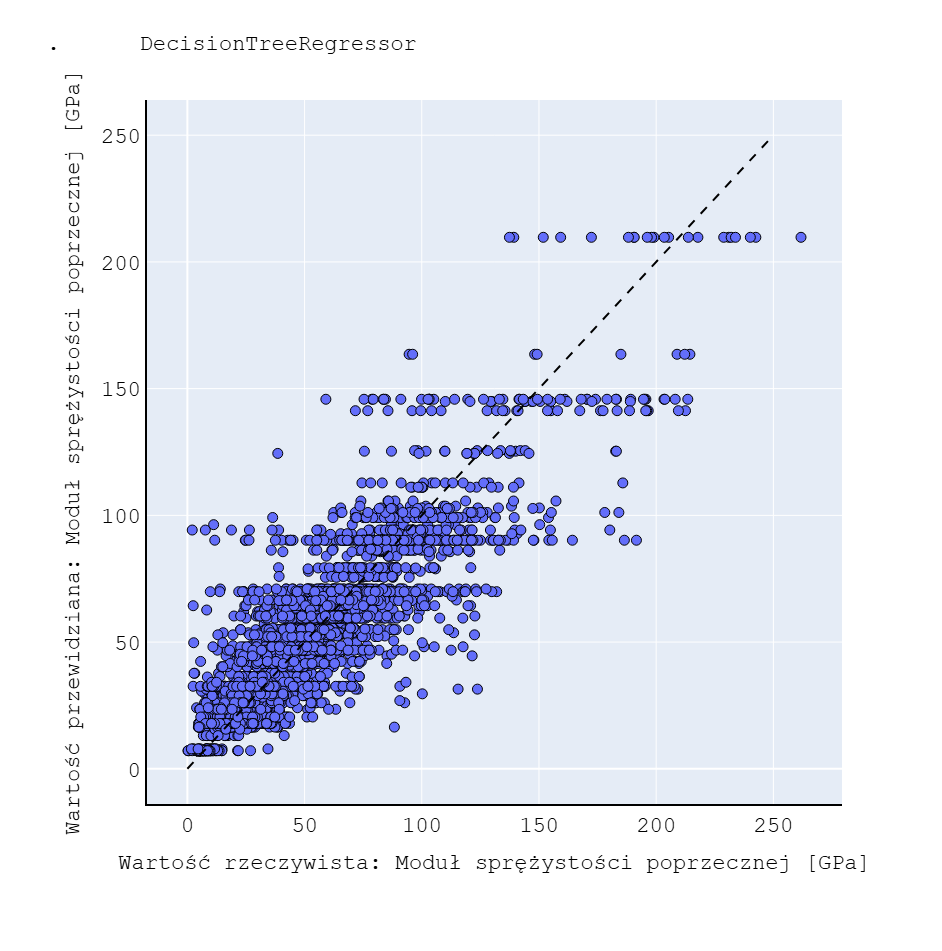
\includegraphics[width=0.48\textwidth]{images/figures/newplot (16).png}
}
\\
\subfigure[Współczynninik Anizotropii]{%
    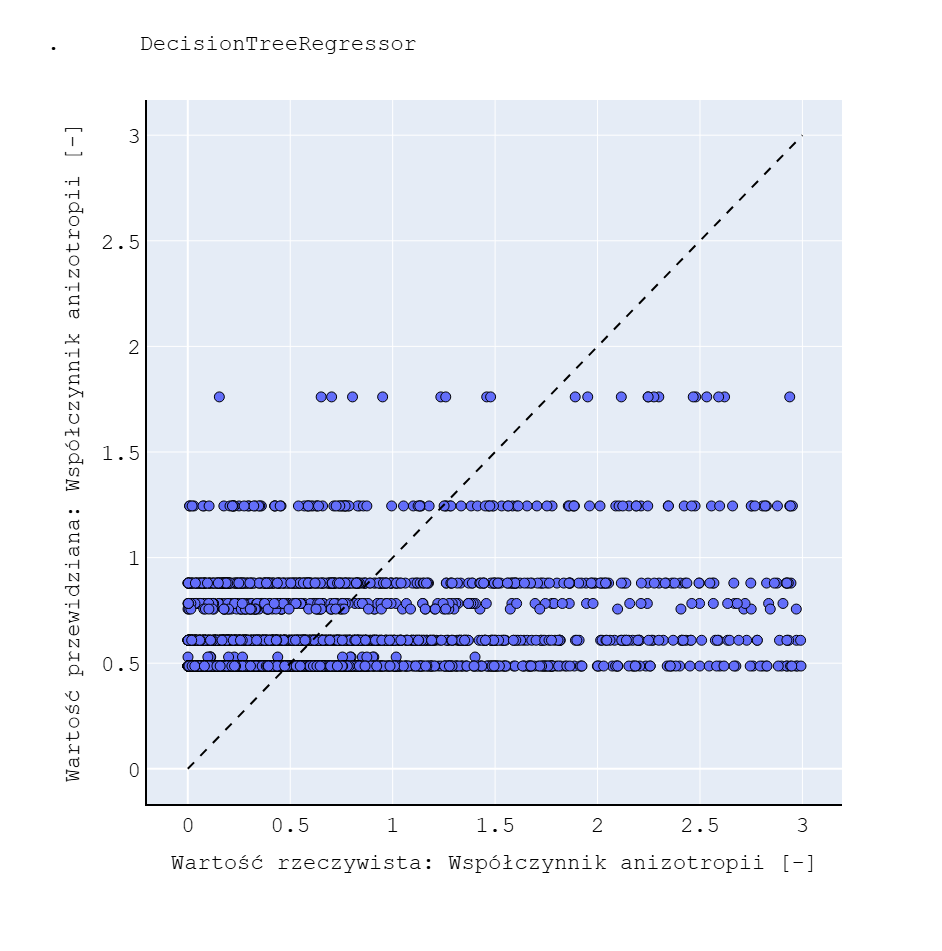
\includegraphics[width=0.48\textwidth]{images/figures/newplot (25).png}
}
\subfigure[Liczba Poisona]{%
    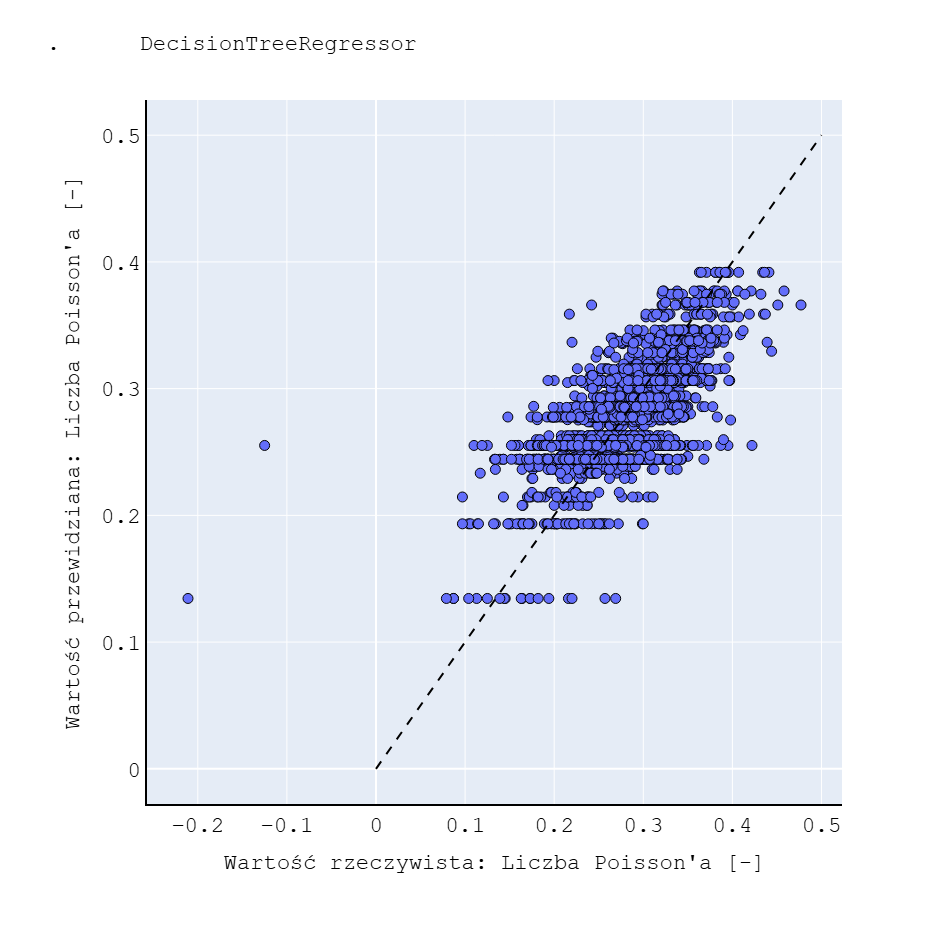
\includegraphics[width=0.48\textwidth]{images/figures/newplot (34).png}
}
\caption{Regresor Drzewa Decyzyjnego}
\end{figure}

opis

\clearpage